\chapter{Potential Outcomes}
\label{ch-pot-out}
This chapter
is based on Ref.\cite{book-mixtape},
a book by Stephen Cunningham entitled 
``Causal inference: the mixtape".

The theory of potential
outcomes (PO) was for the most part
invented in a seminal
1974 paper by Donald B. Rubin. Rubin
has also
made important extensions
to PO theory since 1974. However, he 
does not
use Pearl's causal DAGs to discuss PO theory. 
Pearl has shown that PO theory
can be substantially clarified
and extended by using
the language of causal DAGs.
The d-separation theorem and do operator
that we discuss in  Chapters \ref{ch-dsep}
and \ref{ch-pot-out}
are especially
useful in this regard.
In this chapter, we stress the
connection
of PO theory to 
Pearl's causal DAGs
and bnets.

\begin{table}[h!]
\centering
\begin{tabular}{|l|l|l|l|l|}
\hline
\rowcolor[HTML]{ECF4FF} 
$\s$ & $ d^\s$ & $ y^\s$ & $ y^\s(0)$ & $ y^\s(1)$ \\ \hline
Edith & 0 & 5 & 5 & . \\ \hline
Frank & 0 & 7 & 7 & . \\ \hline
George & 0 & 8 & 8 & . \\ \hline
Hank & 0 & 10 & 10 & . \\ \hline
Andy & \cellcolor[HTML]{FFFFC7}1 & 10 & . & 10 \\ \hline
Ben & \cellcolor[HTML]{FFFFC7}1 & 5 & . & 5 \\ \hline
Chad & \cellcolor[HTML]{FFFFC7}1 & 16 & . & 16 \\ \hline
Daniel & \cellcolor[HTML]{FFFFC7}1 & 3 & . & 3 \\ \hline
\end{tabular}
\caption{PO dataset describing whether
individual $\s$
took a treatment dose ($d^\s=1$)
or didn't ($d^\s=0$).
The 
treatment outcome
is measured by the real number $y^\s$.}
\label{tab-pot-out-missing}
\end{table} 

Suppose a {\bf population
of individuals} $\s=0,1,2, \ldots, nsam-1$
is given ($d^\s=1$) or
not given ($d^\s=0$)
a {\bf treatment discrete drug dose} $d^\s$,
and that
the 
 {\bf treatment outcome (i.e., response)}
is measured by
a real number $y^\s$.
Table \ref{tab-pot-out-missing}
gives a possible {\bf PO dataset}
for this scenario.
As you
can see from
that table,
each individual 
either takes a drug
dose or
doesn't,
but not both.
PO theory
can be viewed as a
 {\bf  missing
data (MD) problem}. MD problems are 
discussed in
 Chapter \ref{ch-missing-d}.
However, the PO MD problem 
is much more specialized
than the generic MD problems
discussed in Chapter \ref{ch-missing-d}.
In the PO MD
problem, we can
fill
in the blank cells
by matching
each individual
that took
the drug with
another {\it similar} 
individual that didn't.
We will have much
more to say about
this matching
strategy later in this chapter.

One can define
similar
individuals as 
individuals that have the same
value
for $nx$ features $x^\s=(x^\s_i)_{i=0, 1, \ldots, nx-1}$.
One
can add to Table \ref{tab-pot-out-missing}
 $nx$ extra columns
giving the value of
the feature vector $x^\s$
for each individual.
Members
of a population with
the same $x^\s$ 
are referred to as 
a
{\bf subpopulation or stratum (i.e., layer)}.

In a {\bf randomized clinical trial (RCT)}
\footnote{The term {\bf A/B test}
is often used to mean a RCT
where A and B are the treated and control groups. However,
sometimes the term is used to refer to 
an experiment  that conditions on confounders,
which violates the definition of a RCT,
and is the same as a PO test.},
the effect 
of the variable $x^\s$ on 
the value
of $d^\s$
is eliminated by
randomizing
the population
and therefore
making the effect of $x^\s$
on $d^\s$
average out  to zero.
However,
there are many situations
in which carrying out a RCT is not
possible
or desirable. PO theory is
a way of predicting the
result
of a RCT in situations where
doing a real RCT is not possible
or desirable.

In this chapter, $x^\s$
will be called the confounders.
Implicit throughout this chapter
is the assumption that there are {\bf 
no unmeasured confounders}.
Because if 
there are some unmeasured confounders,
those can
send secret messages 
that influence the value 
that $d^\s$ takes.
This would ruin
the
predictions
of someone trying
to predict the results of a RCT
without
being privy to those secret 
messages.
When there are {\bf some
unmeasured confounders},
it might still be
possible
to
predict the effect of a RCT.
This might be possible
using instrumental variables. See Chapter
\ref{ch-instrumental}
for a discussion
of {\bf instrumental
variables}.


\section{$G$ and $G_{den}$
bnets,
the starting point bnets}


\begin{figure}[h!]
$$
\begin{array}{ccc}
\xymatrix{
&\rvx^\s\ar[dl]\ar[dr]
\\
\rvd^\s\ar[rr]&&\rvy^\s
}
&&
\xymatrix{
u_\rvd\ar[dd]&u_\rvx\ar[d]&u_\rvy\ar[dd]
\\
&\rvx\ar[dl]\ar[dr]
\\
\rvd\ar[rr]&&\rvy
}
\\
\\
G&&G_{den}
\end{array}
$$
\caption{Bnets
$G$ and $G_{den}$
are 
our starting
point in discussing PO theory. 
 $G$ is for 
a single individual $\s$ of the 
population.
Bnet $G_{den}$ is the 
DEN counterpart 
to $G$.
DEN (Deterministic with
External Noise) bnets are discussed in Chapter
\ref{ch-linear-sys}.} 
\label{fig-po-G-start}
\end{figure}

In this chapter, we will
abbreviate
$\rvX\sqsig=\rvX^\s$
for
$X\in \{d, x, y\}$ 
and for $\s=\{0,1,2, \ldots, nsam-1\}$.


For each individual (aka unit, sample) 
$\s=0, 1, 2, \ldots nsam-1$, let:

$\rvd^\s\in\bool$ be the
 treatment discrete drug dose,  1 if treated and 0 if untreated

$\rvy^\s\in \RR$ be the
 treatment potential outcome

$\rvx^\s$ be the column vector of treatment 
confounders 
(aka covariates because they
are often used as covariates (i.e., 
independent
variables) in linear regression.)

Consider bnets $G$ and $G_{den}$
in 
 Fig.\ref{fig-po-G-start}.
$G$ reflects the language
used in Ref.\cite{book-mixtape}
to discuss PO theory. And
$G_{den}$ reflects
the language that Judea Pearl 
prefers to use to discuss PO theory.
Both languages are equivalent. To go from
one language to the other, one need only
perform the following
swaps, where $\rvu$
is the external noise of the DEN bnet.

$\rvX^\s\leftrightarrow \rvX(\rvu)$
for $X\in \{d, x, y\}$.

$P(\s)=\frac{1}{nsam}\leftrightarrow P(u)$

$\sum_\s P(\s) (\cdot)
\leftrightarrow \sum_uP(u) (\cdot)$




The TPMs, printed in blue,
for the bnet
$G$
in Fig.\ref{fig-po-G-start},
are as follows:


\beq\color{blue}
P(x^\s)=
P_{\rvx}(x^\s)
\eeq

\beq\color{blue}
P(d^\s|x^\s)=
P_{\rvd|\rvx}(d^\s|x^\s)
\eeq


\beq\color{blue}
P(y^\s| d^\s, x^\s)=
P_{\rvy|\rvd, \rvx}(y^\s|d^\s, x^\s)
\eeq




Now let:

$\rvd\in\bool$
be the treatment discrete drug dose,  1 if treated and 0 if untreated

$\rvy\in \RR$ be the
 treatment potential outcome

$\rvx$ be the column vector of 
treatment
confounders (aka covariates)


$\rvu=(\rvu_\rvd, 
\rvu_\rvx, \rvu_\rvy)$ be the
external noise

The TPMs, printed in blue,
for the bnet
$G_{den}$
in Fig.\ref{fig-po-G-start},
are as follows:


\beq \color{blue}
P(x|u_\rvx)= \indi(\;\;x=u_\rvx\;\;)
\eeq

\beq\color{blue}
P(d|x, u_\rvd)=
\indi( \;\; d= f_\rvd(x, u_\rvd)
\;\;)
\eeq

\beq\color{blue}
P(y|d,x, u_\rvy)=
\indi( \;\; y= f_\rvy(d,x, u_\rvy)
\;\;)
\label{eq-y-is-fy}
\eeq

If we linearize
 $f_\rvy$ in Eq.(\ref{eq-y-is-fy}),
we get

\beqa
\rvy =
\delta \rvd + \beta \rvx + \rvu_\rvy
\;,
\label{eq-y-is-lin}
\eeqa
where $\delta, \beta\in \RR$.
Assuming
that $\rvx, \rvy\in \RR$
and $\rvd\in \bool$,
Eq.(\ref{eq-y-is-lin}) can be plotted.
The resulting plot
is given in Fig.\ref{fig-po-two-parallel-lines}.
This plot
is a very special
case of the PO problem,
but it gives a crude idea
of the ``effects" $\delta
= y(1)-y(0)$ that PO theory 
gives estimates for.
Any 
individual participating in the experiment
experiences either $y(1)$
or $y(0)$,
but not both.



\begin{figure}[h!]
\centering
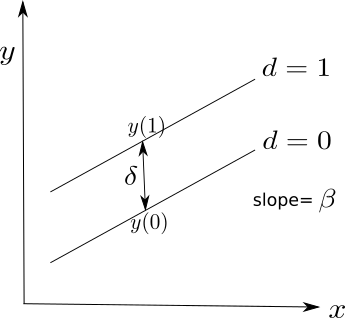
\includegraphics[width=2in]
{pot-out/two-parallel-lines.png}
\caption{Plot  of
Eq.(\ref{eq-y-is-lin})} 
\label{fig-po-two-parallel-lines}
\end{figure}






\section{$G$ bnet
with nodes $y^\sigma(0),
y^\sigma(1)$ added to it.}


\begin{figure}[h!]
$$
\begin{array}{ccccc}
\xymatrix{
&\rvx^\s\ar[ddl]\ar[ddr]
\\
\\
\rvd^\s\ar[rr]&&\rvy^\s
}
&
\xymatrix{
&&\rvx^\s\ar[ddll]\ar[d]
\\
&&[\rvy^\s(0),\rvy^\s(1)]\ar[d]
\\
\rvd^\s\ar[urr]^?\ar[rr]
&
&\rvy^\s
}
\\
G&G_{+}
\end{array}
$$
\caption{
Bnet $G_+$ is bnet $G$
with two new nodes $\rvy^\s(0)$
and $\rvy^\s(1)$
added to it.
The tuple node $[\rvy^\s(0), \rvy^\s(1)]$
can also be represented by
two nodes $\rvc\rarrow\rvy(\rvc)$,
where $\rvc\in \bool$.
} 
\label{fig-po-G-im-y0-y1}
\end{figure}



Consider Fig.\ref{fig-po-G-im-y0-y1}.
Bnet $G_+$
 was obtained by adding two new
nodes $\rvy^\s(0)$
and $\rvy^\s(1)$
to bnet $G$.
The
TPMs, printed in blue,
 for bnet $G_+$,
are as follows. Note
that we define them in terms
of the TPMs
for bnet $G$.

\beq\color{blue}
P(x^\s)=
P_{\rvx}(x^\s)
\eeq

\beq\color{blue}
P(d^\s|x^\s)=
P_{\rvd|\rvx}(d^\s|x^\s)
\eeq

For $c\in \bool$,

\beq\color{blue}
P(y^\s(c)|d^\s, x^\s) = 
\left\{
\begin{array}{ll}
P_{\rvy(c)|\rvd, \rvx}(y^\s(c)|d^\s, x^\s)
& \text{ if INCLUDE arrow  with question mark}
\\
P_{\rvy(c)| \rvx}(y^\s(c)|x^\s)
& \text{ if EXCLUDE arrow wit question mark}
\end{array}
\right.
\eeq

\begin{subequations}
\label{eq-y-equal-ytd}
\beqa\color{blue}
P(y^\s|y^\s(0), y^\s(1), d^\s)=
&=&\color{blue}
\indi(y^\s= d^\s y^\s(1) + (1-d^\s)y^\s(0))
\\
&=&\color{blue}
\indi(y^\s= y^\s(d^\s))
\eeqa
\end{subequations}

Eq.(\ref{eq-y-equal-ytd})
is often referred to as the {\bf SUTVA assumption}.

If we sum over the 
nodes $\rvy(0)$ and $\rvy(1)$
of this bnet, we should
get the bnet $G$.
This is easy to check. Indeed, 

\begin{align}
P(y^\s|d^\s, x^\s)
&=
\sum_{y^\s(0)}
\sum_{y^\s(1)}
\indi(y^\s= y^\s(d^\s))
P(y^\s(0)|d^\s, x^\s)
P(y^\s(1)|d^\s, x^\s)
\\
&=
\left\{
\begin{array}{ll}
P_{\rvy(0)|\rvd, \rvx}(
y^\s|d^\s, x^\s)&\text{ if }
d^\s=0
\\
P_{\rvy(1)|\rvd, \rvx}(
y^\s|d^\s, x^\s)&\text{ if }
d^\s=1
\end{array}
\right.
\;.
\label{eq-y-is-y-td}
\end{align}

Henceforth,
we will refer
to the case where
the question mark
arrow is included as
the general case,
and to the case when it's excluded
as the {\bf weak-d limit}.
Henceforth, we 
will first present
results for the
general case,
and then 
describe how  those
results
change for the
weak-d limit.
Rubinologists
always assume the 
weak-d limit, but
we find that 
with little effort,
we can derive
many results for
general case, and
then compare those 
results 
to their weak-d limit.
I find such
comparisons instructive.

Note that in the general case,
$P(\rvy(c)=y|\rvd=d, x)$
for $c, d\in \bool$
are four 
different probability 
distributions,
and that 
$P(\rvy=y|d=d,x)$
is defined in terms
of two of them, the
so called {\bf factual
distributions} with $c=d$.
By measuring $\rvy$,
we can't access the other
2 probability distributions,
the so called {\bf counter-factual
distributions}
with $c\neq d$.

In the weak-d limit, 
$P(\rvy(c)=y|\rvd=d, x
)=P(\rvy(c)=y|x)$ are 
two probability
distributions, 
and they both
can be accessed 
by measuring $\rvy$.




\section{Expected Values of
 treatment outcome $y^\sigma$}

It is convenient
to define
the following
expected values of
$\rvy^\s$
in terms of the TPMs of
bnet $G_{+}$:

\beq
\caly_{c| d,x}
=
E_{\s| d,x}[\rvy^\s(c)]
\rarrow
E_{ \rvy(c)| d,x} [\rvy(c)]
=\sum_{y} y
P(\rvy(c)=y|\rvd= d,x)
\label{eq-need-positivity}
\eeq

\beq
\caly_{c| d}
=
E_{\s| d}[\rvy^\s(c)]
\rarrow
E_{ \rvy(c)| d} [\rvy(c)]
=\sum_x\caly_{c|d,x}P(x|d)
\eeq

\beq
\caly_{c| x}
=
E_{\s| x}[\rvy^\s(c)]
\rarrow
E_{ \rvy(c)| x} [\rvy(c)]
=\sum_d\caly_{c|d,x}P(d|x)
\eeq


\beq
\caly_c=
E_{\s}[\rvy^\s(c)]
\rarrow
E_{\rvy(c)} [\rvy(c)]=
\sum_{x,d}\caly_{c|d,x} P(x,d)
\eeq

Note that in the weak-d limit,


\beq
\caly_c=\sum_x \caly_{c|d,x}P(x)
\;.
\eeq

Note that in the weak-d limit,
it is seductive to assume that
$\caly_{c|d}=
\sum_x\caly_{c|d,x}P(x)$, 
but that is not how we are
defining 
$\caly_{c|d}$.
In the weak-d limit,
$\caly_{c|d,x}$ is independent
of $d$, but,
if $P(x|d)$ depends on $d$,
then
 $\caly_{c|d}$ depends on $d$ too.
So in the weak-d limit,
$\caly_{c|d, x}$ is independent
of $d$,
but $\caly_{c|d}$
can depend on $d$.


$\caly_{0|0}, \caly_{1|1}$
are said to be {\bf factual} 
(indicating compliant patients)
whereas 
$\caly_{0|1}, \caly_{1|0}$
are said to be {\bf counterfactual} 
(indicating non-compliant patients).

Also let

\beq
\caly_{| d,x}
=
E_{\s| d,x}[\rvy^\s]
\rarrow
E_{\rvy| d,x} [\rvy]
=\sum_{y} y
P(\rvy=y|\rvd= d,x)
\eeq


\beq
\caly_{| d}
=
E_{\s| d}[\rvy^\s]
\rarrow
E_{\rvy| d} [\rvy]
=\sum_x\caly_{|d,x}P(x|d)
\eeq

\beq
\caly_{| x}
=
E_{\s| x}[\rvy^\s]
\rarrow
E_{\rvy| x} [\rvy]
=\sum_d\caly_{|d,x}P(d|x)
\eeq

\beq
\caly
=
E_{\s}[\rvy^\s]
\rarrow
E_{\rvy} [\rvy]
=\sum_d\caly_{|d,x}P(d,x)
\eeq


In the weak-d limit,
$\caly_{|d,x}$ is independent
of $d$, but,
if $P(x|d)$ depends on $d$,
then
 $\caly_{|d}$ depends on $d$ too.
So in the weak-d limit,
$\caly_{|d, x}$ is independent
of $d$,
but $\caly_{|d}$
can depend on $d$.



\section{Translation Dictionary}

\begin{table}[h!]
\renewcommand{\arraystretch}{1.5}
\centering
\begin{tabular}{|l|l|}
\hline
\rowcolor[HTML]{ECF4FF} 
In standard PO notation&
In our notation \\
\hline
$i$, individual (i.e., unit, sample) index& $\s$ \\ 
\hline 
$D_i=d_i$, treatment dose & $\rvd^\s=d^\s$\\
\hline 
$Y_i=y_i$, treatment outcome& $\rvy^\s=y^\s$ \\ 
\hline 
$X_i=x_i$, treatment confounders& $\rvx^\s=x^\s$ \\ 
\hline
$E[Y_i(c)]$ & 
$E_{\s}[\rvy^\s(c)]=\caly_{c}$ \\
\hline
$E[Y_i(c)|D_i= d]$ & 
$E_{\s| d}[\rvy^\s(c)]=\caly_{c| d}$\\
\hline
$E[Y_i(c)|D_i= d, X_i=x]$ & 
$E_{\s| d,x}[\rvy^\s(c)]=\caly_{c| d,x}$\\
\hline
$E[Y_i]$ & 
$E_{\s}[\rvy^\s]=\caly$ \\
\hline
$E[Y_i|D_i= d]$ & 
$E_{\s| d}[\rvy^\s]=\caly_{| d}$\\
\hline
$E[Y_i|D_i= d, X_i=x]$ & 
$E_{\s| d,x}[\rvy^\s]=\caly_{| d,x}$\\
\hline
\end{tabular}
\caption{Dictionary for 
translating
from standard PO notation
of Ref.\cite{book-mixtape} to our notation.
}
\label{tab-pot-out-dict}
\end{table}
\renewcommand{\arraystretch}{1}

Table \ref{tab-pot-out-dict}
gives a dictionary for 
translating
from the standard PO notation 
of Ref.\cite{book-mixtape}
to our notation. $c, d\in \bool$.


\section{${\cal Y}_{|d,x}
={\cal Y}_{d|d,x}$ (SUTVA)}


\begin{claim}\footnote{In the
standard PO notation,
this is the frequently used identity 
$$E[Y|D=d, x]= E[Y(d)|D=d, x]$$.
}
\label{cl-caly-bardx}

\beq
\caly_{| d, x}=\caly_{ d| d,x}
\label{eq-y-to-yd-x}
\eeq

\beq
\caly_{| d}=\caly_{ d| d}
\label{eq-y-to-yd}
\eeq

\end{claim}
\proof

\beqa
\caly_{| d,x}
&=&
\sum_y y P(\underbrace{\rvy}_
{=\rvy( d) 
\text{ by Eq.(\ref{eq-y-equal-ytd})}}
=y| d, x)
\\
&=&
\caly_{ d| d, x}
\;.
\eeqa
Applying $\sum_x P(x|d)$ to
both sides 
of Eq.(\ref{eq-y-to-yd-x})
gives
Eq.(\ref{eq-y-to-yd})
\qed



\section{Conditional Independence Assumption (CIA)}

The {\bf Conditional Independence Assumption}
 (CIA)
is said to hold 
 if
\beq
(\rvy^\s(0), \rvy^\s(1),
\rvy^\s)\perp_P\rvd^\s | \rvx^\s
\;.
\label{eq-CIA2}
\eeq
This is satisfied by $G_+$
in the weak-d limit. To
prove this, check that

\beq
(\rvy^\s(0),\rvy^\s(1),
\rvy^\s)
\perp_{G_{+}} \rvd^\s|\rvx^\s
\;
\eeq
and then invoke
the d-separation theorem 
(see Chapter \ref{ch-dsep}).

I think CIA only makes sense
if the individuals 
are treatment blind (i.e., 
have no knowledge
of whether they are
in the treated or control
groups.) Otherwise,
that extra knowledge 
becomes a
confounder not being
included in $x$.

A {\bf Randomized Control Trial (RCT)}
is defined to satisfy
Eq.(\ref{eq-CIA2}) without the
 $\rvx^\s$ conditioning; i.e., it 
satisfies

\beq
(\rvy^\s(0), \rvy^\s(1),
\rvy^\s)\perp_P\rvd^\s 
\;.
\label{eq-CIA-minus-x}
\eeq
This means that in a RCT,
the arrow from 
$\rvx^\s$ to  $\rvd^\s$ in $G_+$
is omitted.

Note that
if we assume both CIA (i.e.,
weak-d limit)
and SUTVA, we get 

\begin{subequations}
\beqa
\caly_{|d,x}
&=&
E_{\s|d,x}[\rvy^\s]
\\
&=&
E_{\s}[\rvy^\s|\rvd^\s=d, \rvx^\s=x]
\\
&=&
E_{\s}[\rvy^\s(d)|\rvd^\s=d, \rvx^\s=x]
\text{ (by SUTVA)}
\\
&=&
E_{\s}[\rvy^\s(d)|\rvx^\s=x]
\text{ (by CIA)}
\\
&=&
E_{\s|x}[\rvy^\s(d)]
\\
&=&
\caly_{d|x}
\;.
\label{eq-d-td-diff}
\eeqa
\end{subequations}
In a RCT, Eq.(\ref{eq-d-td-diff})
is valid without the $x$ conditioning.


\section{Treatment Effects}

\begin{figure}[h!]
\centering
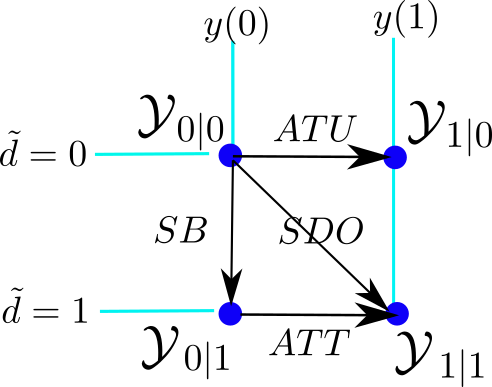
\includegraphics[height=1.8in]
{pot-out/y-diffs-square.png}
\caption{Different treatment effects.  
A treatment effect is a difference of 
two $\caly_{c| d }$.} 
\label{fig-y-diffs-square}
\end{figure}

A {\bf treatment effect} is a
a difference of two  $\caly_{c| d }$.
It is convenient to
define the following 
treatment effects. 
See Fig.\ref{fig-y-diffs-square}.
In that figure, $y(c)$ appears  with
$c=0,1$.




\begin{itemize}


\item average treatment effect
 (ATE).
\beq
{\color{red}ATE}=
\caly_{1}-
\caly_{0}= \delta
\eeq

\item average treatment effect 
of the treated (ATT)
\beq
{\color{red}ATT}=
\caly_{1|1}-\caly_{0|1}
\eeq


\item average
treatment effect of the untreated (ATU)
\beq
{\color{red}ATU}=
\caly_{1|0}-\caly_{0|0}
\eeq

\item selection bias (SB)
\beq
{\color{red}SB}=\caly_{0|1}-\caly_{0|0}
\eeq


\item simple difference in outcomes (SDO)
\beq
{\color{red} SDO}= \caly_{1|1}-\caly_{0|0}
\eeq


\end{itemize}



Let

\beq
\pi_d = P(\rvd=d)
\eeq
for $d\in \bool$.

Note that there
exist some linear 
constraints between 
these treatment effects.



\beqa
\underbrace{\caly_1-\caly_0}_
{ATE}
&=&
\underbrace{
\caly_{1|1}\pi_1 +\caly_{1|0}\pi_0}_
{\caly_1}
-
\underbrace{(
\caly_{0|1}\pi_1 + \caly_{0|0}\pi_0)}_
{\caly_0}
\\
&=&
 \underbrace{(\caly_{1|1}-\caly_{0|1})}_{ATT}\pi_1+
 \underbrace{(\caly_{1|0}-\caly_{0|0})}_{ATU}\pi_0
\label{eq-ate-att-atu}
\eeqa

\beq
\underbrace{\caly_{1|1}-\caly_{0|0}}_{SDO}
=
\underbrace{(\caly_{1|1}-\caly_{0|1})}_{ATT}
+
\underbrace{\caly_{0|1}-\caly_{0|0}}_{SB}
\eeq

\beqa
\underbrace{\caly_{1|1}-\caly_{0|0}}_{SDO}
&=&
\underbrace{(\caly_{1|1}-\caly_{0|1})\pi_1 +
(\caly_{1|0}-\caly_{0|0})\pi_0 }_{ATE} \nonumber
\\
&&+
\underbrace{\caly_{0|1}-\caly_{0|0}}_{SB}\nonumber
\\
&&+
\underbrace{(\caly_{1|1}-\caly_{0|1})}_{ATT}\pi_0\nonumber
\\
&&-
\underbrace{(\caly_{1|0}-\caly_{0|0})}_{ATU}\pi_0
\label{eq-sdo-ate-else}
\eeqa

By virtue of  Eq.(\ref{eq-ate-att-atu}),

\beq
ATT=ATU\implies ATT=ATU=ATE
\;
\eeq
and

\beq
ATE=0 \iff \frac{ATU}{ATT}=-\left(\frac{\pi_1}{\pi_0}\right)
\;.
\eeq
Whenever
$ATT=ATU$,
we will say there
is {\bf T-U symmetry}.


In general, $SDO=ATT+SB$, but if there is 
T-U symmetry,
then $SDO=ATE+SB$. 

If there is T-U symmetry  and 
zero bias  $SB=0$, 
then $SDO=ATE=ATT=ATU$.

If there is a
null result 
for a RCT (i.e., $ATE=0$),
T-U symmetry 
and zero bias $SB=0$, 
then
$SDO=ATE=ATT=ATU=0$.


Let

\beq
\caly_{c,d|x}=\caly_{c|d,x}P(d|x)
\eeq
Every $\cale \in\{ATE,ATT,ATU,SB, SDO\}$
can be 
defined for a fixed stratum $x$
by replacing each $\caly_{c| d }$
with  $\caly_{c, d | x}$. 
For example, 
\beq
ATT=\caly_{1|1}-\caly_{0|1}\text{ so }
ATT_x=\caly_{1,1|x}-\caly_{0,1|x}
\;.
\eeq
We will denote this stratum restricted
version of $\cale$ by $\cale_x$.
We can calculate $\cale$ using

\beq
\cale=E_x[\cale_x]=
\sum_x P(x) \cale_x
\;.
\eeq




\section{Insights into 
what makes treatment effects equal and 
$\caly_{1|0}=\caly_{1}$}
\label{sec-td-ignored}

\begin{figure}[h!]
\centering
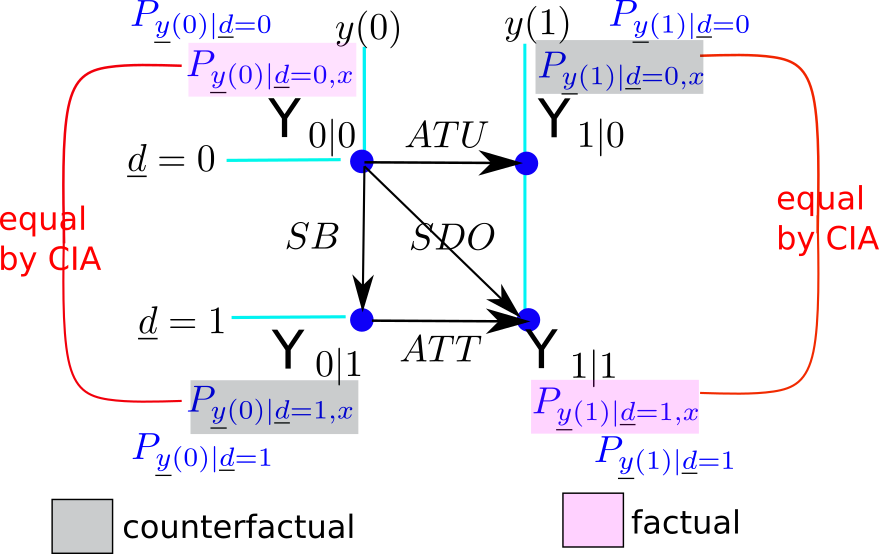
\includegraphics[width=4in]
{pot-out/y-diffs-square-probs.png}
\caption{Figure \ref{fig-y-diffs-square} 
with added information
about  probability distributions 
used to obtain each expected value
 $\caly_{c| d }$.}
\label{fig-y-diffs-square-probs}
\end{figure}


\begin{enumerate}
\item 
Is it
possible for $SDO=0$ but $ATE\neq 0$
or vice versa, and
what is going on when this is true?
\item
What is going on when two treatment effects
are equal; for instance, when $ATT=ATU$?
\item
When is $\caly_{1|0}=\caly_{1}$,
and what is going on when this is  true?
\end{enumerate}
Fig.\ref{fig-y-diffs-square-probs}
gives some 
intuition 
about what is
going on when any of these 
things happen.

Recall that
each expected value
$\caly_{c|d}$ 
is associated with a probability
distribution $P_{\rvy(c)|\rvd,x}$.

\beq
\caly_{c| d }
=
\sum_{y} y 
\underbrace{\sum_x 
P_{\rvy(c)| \rvd,x}(y| d,x)P(x|d)}_{
P_{\rvy(c)| \rvd}(y| d)}
\eeq
for $c,  d\in \bool$.
Fig.\ref{fig-y-diffs-square-probs}
reminds us of which $P$
is used to generate each $\caly$.
From this figure, we see that

\begin{enumerate}
\item
A sufficient
condition for $SDO=0$
is that 
$P_{\rvy(1)| \rvd=1,x}
=
P_{\rvy(0)| \rvd=0,x}$.
A sufficient
condition for $ADE=0$
is that 
$P_{\rvy(1)|x}
=
P_{\rvy(0)|x}$.

\item
A sufficient condition for
$ATT=ATU$
is that 
$P_{\rvy(1)| \rvd=0,x}
-
P_{\rvy(0)| \rvd=0,x}$
equals
$P_{\rvy(1)| \rvd=1,x}
-
P_{\rvy(0)| \rvd=1,x}$.
\item
A sufficient condition for $\caly_{1|0}=\caly_{1}$
is that
$P_{\rvy(1)| \rvd=0}=
P_{\rvy(1)}$. Note that
the CIA implies that 
$P_{\rvy(1)| \rvd=0,x}=
P_{\rvy(1)|x}$ always,
but this does not imply that
$P_{\rvy(1)| \rvd=0}=
P_{\rvy(1)}$.
\end{enumerate}


\section{$G_{do+}$  bnet}
\begin{figure}[h!]
$$
\begin{array}{ccccc}
\xymatrix{
&\rvx^\s\ar[dr]\ar[dl]
\\
\rvd^\s\ar[rr]&&\rvy^\s
}
&&
\xymatrix{
&\rvx^\s\ar[dr]
\\
\rho\rvd^\s=\td^\s\ar[rr]&&\rvy^\s
}
&&
\xymatrix{
&\rvx^\s\ar[dr]
\\
\rho\rvd^\s\ar[rr]&&\rvy^\s
}
\\
\\
G&&G_{do}= \rho_{\rvd^\s}
(\td^\s)G&& G_{do+}
\end{array}
$$
\caption{Bnet $G_{do}= \rho_{\rvd^\s}
(\td^\s)G$
is obtained by applying
the do operator to node $\rvd^\s$
of bnet $G$. Bnet $ G_{do+}$
is obtained
by adding a prior
probability distribution $P(\td^\s)$
to node $\rho\rvd^\s$ of
bnet $G_{do}$.}
\label{fig-po-G-do}
\end{figure}

Fig.\ref{fig-po-G-do}
shows how bnet $G_{do}$
is obtained by applying
the do operator to bnet $G$,
and
how
bnet $G_{do+}$
is obtained by adding
a prior
probability distribution
 to one of the nodes
of $G_{do}$.
In bnet $G_{do}$,
node  $\rvd^\s$ has been
stripped of all outside
influences and fixed to a
specific state $\td^\s$.
This is what a RCT does.

The TPMs, printed in blue,
for the bnets $G_{do}$
and $G_{do+}$,
are as follows.
Note that the TPMs
for bnets  $G_{do}$ and $G_{do+}$
are defined in terms
of the TPMs of bnet $G$.

\beq\color{blue}
P(x^\s)=
P_{\rvx}(x^\s)
\eeq

\beq
P_{\rho\rvd}(\td)=\sum_x P_{\rvd|\rvx}
(\td|x)P_\rvx(x)
\eeq

\beq\color{blue}
P((\td^\s)')=
\left\{
\begin{array}{ll}
\delta(\td^\s, (\td^\s)')& \text{for $G_{do}$}
\\
P_{\rho\rvd}(\td^\s)
& \text{for $G_{do+}$}
\end{array}
\right.
\eeq

\beq\color{blue}
P(y^\s|\td^\s, x^\s)=
P_{\rvy|\rvd, \rvx}(y^\s|\td^\s, x^\s)
\eeq

Note that in $G_{do}$,

\beq
P(\rvy=y|\rho \rvd=d, \rvx=x)=
P(y|\rvd=d,x)
\;
\label{eq-rho-begone}
\eeq
because, by the d-separation
theorem,  when we condition on
the confounder $\rvx$, 
we  block information from being
transmitted from $\rvd$ to $\rvy$ through $\rvx$,
and this is equivalent to
amputating the arrow $\rvx\rarrow\rvd$.

Using Eq.(\ref{eq-rho-begone}), we get

\beqa
P(\rvy=y|\rho\rvd=d)
&=&
\sum_x 
P(\rvy=y|\rho\rvd=d, x)P(x|\rho\rvd=d)
\\
&=&
\sum_x 
P(y|d, x)P(x)
\label{eq-po-backdoor}
\eeqa
Eq.(\ref{eq-po-backdoor})
is called the {\bf backdoor criterion formula}.
It allows us to
express a
probability
with a do operator
in terms 
of  probabilities
without do operators.

\section{$ACE=ATE$}



Define the Average
Causal Effect ($ACE$) by

\begin{align}
ACE&=\sum_y y
[P(y|\rho\rvd=1)-P(y|\rho\rvd=0)]
\\
&=
\sum_x P(x)\sum_y y [P(y|\rvd=1,x)-P(y|\rvd=0,x)]
\;. \text{ (by Eq.(\ref{eq-po-backdoor})}
\label{eq-my-backdoor-proof} 
\end{align}


\begin{claim}\label{cl-ace-ate}
If we assume both SUTVA and 
CIA (i.e., weak-d limit), then
\beq
ACE=ATE
\eeq
\end{claim}
\proof



\begin{align}
ACE&=
\sum_x P(x)\sum_y y [P(\rvy=y|\rvd=1,x)-
P(\rvy=y|\rvd=0,x)] 
\\
&=\sum_x P(x)[\caly_{1|1, x}-\caly_{0|0, x}]
\;\text{(by SUTVA)}
\\
&=\sum_x P(x)[\caly_{1|x}-\caly_{0|x}]
\;\text{(by CIA)}
\\
&=
\caly_{1}-\caly_{0}
\\
&=
ATE
\end{align}
\qed

We will say there is a {\bf null result
in a RCT} when $ACE=0$. By the previous claim, 
this is true iff $ATE=0$
(assuming weak-d limit).

\section{$(SDO,ATE)$ space}
If we substitute
$y^\s\rarrow y^\s( d^\s)$ and
 $y^{m(\s)}\rarrow y^\s(1-d^\s)$ 
into 
the estimator
Eq.(\ref{eq-est-ate}) for $ATE$
and the estimator
Eq.(\ref{eq-est-sdo}) for $SDO$,
we get

\beqa
\widehat{ATE}_x
&=&
\frac{1}{N_x}\sum_{\s\in A_x}
 (2 d^\s-1)[y^\s( d^\s) -y^\s(1-d^\s)]
\\
&=&
\frac{1}{N_x}\sum_{\s\in A_x}
 [y^\s(1) -y^\s(0)]
\label{eq-est-ate-simple}
\eeqa
and

\beqa
\widehat{SDO}_x
&=&
\frac{1}{N_{1,x}}
\sum_{\s\in A_x}  d^\s y^\s( d^\s)
-
\frac{1}{N_{0,x}}
\sum_{\s\in A_x} (1- d^\s) y^\s( d^\s)
\\
&=&
\frac{1}{N_{1,x}}
\sum_{\s\in A_{1,x}} y^\s(1)
-
\frac{1}{N_{0,x}}
\sum_{\s\in A_{0,x}}  y^\s(0)
\;.
\label{eq-est-sdo-simple}
\eeqa  

Recall that 
$\hat{\cale}=E_x[\hat{\cale}_x]=
\sum_x \frac{N_x}{N}\hat{\cale}_x$
for $\cale\in\{ATE, SDO\}$.

Recall also that 
$ACE=ATE=0$ is the null 
result in a RCT. 


Suppose that
the treatment outcome $y^\s$
has only two 
possible values, 0 and 1.
Then, $-1\leq ATE \leq 1$
and
$-1\leq SDO \leq 1$.
But does  $ATE=0$
imply $SDO=0$
or vice versa?
Next, we answer 
that question
and more
by finding
the region
of accessibility in the
$(SDO, ATE)$
plane,
assuming $y^\s\in \bool$.


\newpage

\begin{figure}[h!]
\centering
\subfloat[$ATE=-1$ $(SDO=-1)$ point A]{
\begin{tabular}{|
>{\columncolor[HTML]{ECF4FF}}l |l|l|l|}
\hline
\cellcolor[HTML]{CBCEFB}$\s$ & \cellcolor[HTML]{CBCEFB}$ d^\s$ & \cellcolor[HTML]{CBCEFB}$y^\s(0)$ & \cellcolor[HTML]{CBCEFB}$y^\s(1)$ \\ \hline
1 & 0 & 1 & 0 \\ \hline
2 & 0 & 1 & 0 \\ \hline
3 & 0 & 1 & 0 \\ \hline
4 & 1 & 1 & 0 \\ \hline
5 & 1 & 1 & 0 \\ \hline
6 & 1 & 1 & 0 \\ \hline
\end{tabular}
}
\quad
\subfloat[$ATE=\frac{1}{2}$ $(SDO=0)$ point B]{
\begin{tabular}{|
>{\columncolor[HTML]{ECF4FF}}l |l|l|l|}
\hline
\cellcolor[HTML]{CBCEFB}$\s$ & \cellcolor[HTML]{CBCEFB}$ d^\s$ & \cellcolor[HTML]{CBCEFB}$y^\s(0)$ & \cellcolor[HTML]{CBCEFB}$y^\s(1)$ \\ \hline
1 & 0 & 0 & 1 \\ \hline
2 & 0 & 0 & 1 \\ \hline
3 & 0 & 0 & 1 \\ \hline
4 & 1 & 0 & 0 \\ \hline
5 & 1 & 0 & 0 \\ \hline
6 & 1 & 0 & 0 \\ \hline
\end{tabular}
}
\quad
\subfloat[$ATE=1$ $(SDO=1$) point C]{
\begin{tabular}{|
>{\columncolor[HTML]{ECF4FF}}l |l|l|l|}
\hline
\cellcolor[HTML]{CBCEFB}$\s$ & \cellcolor[HTML]{CBCEFB}$ d^\s$ & \cellcolor[HTML]{CBCEFB}$y^\s(0)$ & \cellcolor[HTML]{CBCEFB}$y^\s(1)$ \\ \hline
1 & 0 & 0 & 1 \\ \hline
2 & 0 & 0 & 1 \\ \hline
3 & 0 & 0 & 1 \\ \hline
4 & 1 & 0 & 1 \\ \hline
5 & 1 & 0 & 1 \\ \hline
6 & 1 & 0 & 1 \\ \hline
\end{tabular}
}
\caption{Examples of PO datasets. Exploring $ATE$ extremes.}
\label{fig-ate-possi}
\end{figure}

\begin{figure}[h!]
\centering
\subfloat[$SDO=-1$ $(ATE=0)$ point D]{
\begin{tabular}{|
>{\columncolor[HTML]{ECF4FF}}l |l|l|l|}
\hline
\cellcolor[HTML]{CBCEFB}$\s$ & \cellcolor[HTML]{CBCEFB}$ d^\s$ & \cellcolor[HTML]{CBCEFB}$y^\s(0)$ & \cellcolor[HTML]{CBCEFB}$y^\s(1)$ \\ \hline
1 & 0 & 1 & 1 \\ \hline
2 & 0 & 1 & 1 \\ \hline
3 & 0 & 1 & 1 \\ \hline
4 & 1 & 0 & 0 \\ \hline
5 & 1 & 0 & 0 \\ \hline
6 & 1 & 0 & 0 \\ \hline
\end{tabular}
}
\quad
\subfloat[$SDO=0$ $(ATE=-\frac{1}{2})$ point E]{
\begin{tabular}{|
>{\columncolor[HTML]{ECF4FF}}l |l|l|l|}
\hline
\cellcolor[HTML]{CBCEFB}$\s$ & \cellcolor[HTML]{CBCEFB}$ d^\s$ & \cellcolor[HTML]{CBCEFB}$y^\s(0)$ & \cellcolor[HTML]{CBCEFB}$y^\s(1)$ \\ \hline
1 & 0 & 1 & 0 \\ \hline
2 & 0 & 1 & 0 \\ \hline
3 & 0 & 1 & 0 \\ \hline
4 & 1 & 1 & 1 \\ \hline
5 & 1 & 1 & 1 \\ \hline
6 & 1 & 1 & 1 \\ \hline
\end{tabular}
}
\quad
\subfloat[$SDO=1$ $(ATE=0$) point F]{
\begin{tabular}{|
>{\columncolor[HTML]{ECF4FF}}l |l|l|l|}
\hline
\cellcolor[HTML]{CBCEFB}$\s$ & \cellcolor[HTML]{CBCEFB}$ d^\s$ & \cellcolor[HTML]{CBCEFB}$y^\s(0)$ & \cellcolor[HTML]{CBCEFB}$y^\s(1)$ \\ \hline
1 & 0 & 0 & 0 \\ \hline
2 & 0 & 0 & 0 \\ \hline
3 & 0 & 0 & 0 \\ \hline
4 & 1 & 1 & 1 \\ \hline
5 & 1 & 1 & 1 \\ \hline
6 & 1 & 1 & 1 \\ \hline
\end{tabular}
}
\caption{Examples of PO datasets. Exploring $SDO$ extremes.}
\label{fig-sdo-possi}
\end{figure}

\begin{figure}[h!]
\centering
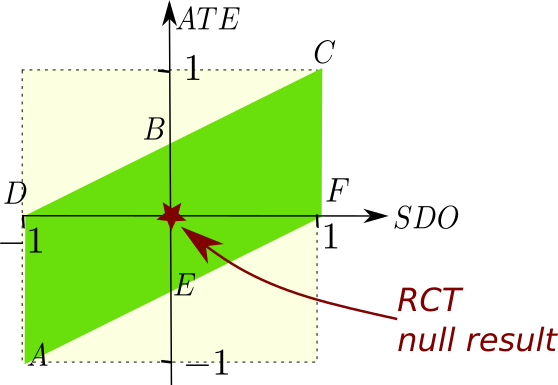
\includegraphics[width=2.5in]
{pot-out/sdo-ate-polytope.png}
\caption{
Green parallelogram
is accessible region in
$(SDO,ATE)$ plane,
assuming $y^\s\in \bool$.
Each of the
six points A, B, \ldots F
corresponds to one of the six tables
in Figs. \ref{fig-ate-possi}
and \ref{fig-sdo-possi}.
Segment $DF$ 
corresponds to the null
result in a RCT. 
} 
\label{fig-sdo-ate-polytope}
\end{figure}



\section{Strata-Matching}

For a situation
described by
the bnet $G_{+}$
\ul{ in the weak-d limit},
we can match {\it similar}
individuals to fill the blank cells of
 Table \ref{tab-pot-out-missing}.
By ``similar", we mean that
they have the same or almost the same
value of $\rvx^\s$.

The reason the weak-d limit
is required is because
it implies that $P(y(c)|d=0,x)=
P(y(c)|d=1,x)$ for $c\in \bool$,
Hence, we can sample from a 
known factual $(c=d)$
distribution to
fill  the missing data
in the unknown counterfactual $(c\neq d)$
distribution.





\subsection{Exact   strata-matching}

\subsubsection{Estimates of Treatment Effects}
\label{sec-estimates}
For $ d\in \bool$ and all strata $x$,
define the sets of individuals
$A_{ d,x}=\{\s:  d^\s= d, x^\s=x\}$,
$A_x=A_{0,x}\cup A_{1,x}$ and $A=\cup_x A_x$.
Let $N_{ d,x}=|A_{ d,x}|$,
$N_x= |A_x|$ and $N=|A|$.

In an exact   strata-matching,
we match each individual with
$ d^\s=d, x^\s=x$
with
exactly
one individual
with $ d^\s=1-d, x^\s=x$.
Define a map $m:A\rarrow A$
such that,
for each $x$, and
for $d\in \bool$,
if $\s\in A_{d,x}$, then
$m(\s)\in A_{1-d,x}$ 
This assumes $A_{0,x}$ and $A_{1,x}$
are non-empty for all $x$.
The purpose of map $m()$
is
to fill in the missing data in the
PO dataset. See Fig.\ref{tab-po-s-map}
for a pictorial representation of 
this.

\begin{table}[h!]
\centering
\begin{tabular}{|l|l|l|}
\hline
 & \cellcolor[HTML]{ECF4FF}$y^\s(0)$ & \cellcolor[HTML]{ECF4FF}$y^\s(1)$ \\ \hline
\cellcolor[HTML]{ECF4FF}$ d^\s=0$ & $y^\s$ & $y^{m(\s)}$ \\ \hline
\cellcolor[HTML]{ECF4FF}$ d^\s=1$ & $y^{m(\s)}$ & $y^\s$ \\ \hline
\end{tabular}
\caption{Illustration of the
purpose of the map $m()$.
Note that $y^\s=y^\s( d^\s)$
 and $y^{m(\s)}=y^\s(1-d^\s)$.}
\label{tab-po-s-map}
\end{table}



Note that
\beq
\sum_{\s\in A_{x}}\frac{ d^\s}{N_{1,x}}=
\sum_{\s\in A_{1,x}}\frac{1}{N_{1,x}}=1
\;.
\eeq
Thus

\beq
\sum_{\s\in A_{x}}\frac{ d^\s}{N_{1,x}}y^\s=
E_{\s| d=1,x}[y^\s]=\caly_{1|1,x}
\eeq
Table \ref{tab-po-yc-at-dx}
gives
estimates of
$ \caly_{c| d ,x}$

{\renewcommand{\arraystretch}{1.5}
\begin{table}[h!]
\centering
\begin{tabular}{|l|l|l|}
\hline
 & \cellcolor[HTML]{ECF4FF}$y^\s(0)$ 
& \cellcolor[HTML]{ECF4FF}$y^\s(1)$ 
\\ \hline
\cellcolor[HTML]{ECF4FF}$ d^\s=0$ 
& 
$\frac{1}{N_{0,x}}\sum_{\s\in A_x} (1- d^\s)y^{\s}=\caly_{0|0,x}$
& 
$\frac{1}{N_{0,x}}\sum_{\s\in A_x} (1- d^\s) y^{m(\s)}=\caly_{1|0,x}$
\\ \hline
\cellcolor[HTML]{ECF4FF}$ d^\s=1$ 
&
 $\frac{1}{N_{1,x}}\sum_{\s\in A_x}  d^\s y^{m(\s)}=\caly_{0|1,x}$
& 
$\frac{1}{N_{1,x}}\sum_{\s\in A_x}  d^\s y^\s=\caly_{1|1,x}$
\\ \hline
\end{tabular}
\caption{Estimates of
$ \caly_{c| d ,x}$.}
\label{tab-po-yc-at-dx}
\end{table}}

{\renewcommand{\arraystretch}{1.5}
\begin{table}[h!]
\centering
\begin{tabular}{|l|l|l|}
\hline
 & \cellcolor[HTML]{ECF4FF}$y^\s(0)$ 
& \cellcolor[HTML]{ECF4FF}$y^\s(1)$ 
\\ \hline
\cellcolor[HTML]{ECF4FF}$ d^\s=0$ 
& 
$\frac{1}{N_{x}}\sum_{\s\in A_x} 
(1- d^\s)y^{\s}=\caly_{0,0|x}$
& 
$\frac{1}{N_{x}}\sum_{\s\in A_x}
 (1- d^\s) y^{m(\s)}=\caly_{1,0|x}$
\\ \hline
\cellcolor[HTML]{ECF4FF}$ d^\s=1$ 
&
 $\frac{1}{N_{x}}\sum_{\s\in A_x} 
 d^\s y^{m(\s)}=\caly_{0,1|x}$
& 
$\frac{1}{N_{x}}\sum_{\s\in A_x} 
 d^\s y^\s=\caly_{1,1|x}$
\\ \hline
\end{tabular}
\caption{Estimates of
$ \caly_{c, d| x}$.}
\label{tab-po-ycd-at-x}
\end{table}}


Recall that

\beq
\caly_{c,d|x}=\caly_{c|d,x}P(d|x)
\eeq
Hence,

\beqa
\caly_{c,d|x}
&=&
(N_{d,x}\caly_{c|d,x})
\frac{P(d|x)}{N_{d,x}}
\\
&=&
(N_{d,x}\caly_{c|d,x})
\frac{1}{N_x}
\eeqa
Table \ref{tab-po-ycd-at-x}
gives
estimates of
$ \caly_{c, d |x}$


The treatment effects $\cale=
ATE, ATT, ATU, SB, SDO$
can be estimated from the data
via the following estimators.



\beqa
\widehat{ATE}_x
&=&
\overbrace{
\caly_{1|1,x}P(1|x) +
 \caly_{1|0,x}P(0|x)}^
{\caly_{1|x}}
-
\overbrace{(
\caly_{0|1,x}P(1|x) +
\caly_{0|0,x}P(0|x))}^
{\caly_{0|x}}
\\
&=&
\frac{1}{N_x}[
\widehat{ATT}_x N_{1,x} +
\widehat{ATU}_x N_{0,x}]
\\
&=&
\frac{1}{N_x}
\left[\sum_{\s\in A_x}  d^\s [y^\s - y^{m(\s)}]+
\sum_{\s\in A_x}(1- d^\s) [ y^{m(\s)}-y^\s]
\right]
\\
&=&
\frac{1}{N_x}\sum_{\s\in A_x} (2 d^\s-1)[y^\s -y^{m(\s)}]
\label{eq-est-ate}
\eeqa

\beqa
\widehat{ATT}_x
&=&
\overbrace{\frac{1}{N_{x}}
\sum_{\s\in A_x}  d^\s y^\s}
^{\caly_{1,1|x}}
 - 
\overbrace{\frac{1}{N_{x}}
\sum_{\s\in A_x}  d^\s y^{m(\s)}}
^{\caly_{0,1|x}}
\\
&=&
\frac{1}{N_{x}}\sum_{\s\in A_x} 
 d^\s [y^\s - y^{m(\s)}]
\label{eq-est-att}
\eeqa


\beqa
\widehat{ATU}_x
&=&
\overbrace{\frac{1}{N_{x}}
\sum_{\s\in A_x} (1- d^\s) y^{m(\s)} }
^{\caly_{1,0|x}}
 - 
\overbrace{\frac{1}{N_{x}}
\sum_{\s\in A_x} (1- d^\s)y^\s}
^{\caly_{0,0|x}}
\\
&=&
\frac{1}{N_{x}}\sum_{\s\in A_x} (1- d^\s) [ y^{m(\s)}-y^\s]
\label{eq-est-atu}
\eeqa

\beq
\widehat{SB}_x =
\overbrace{\frac{1}{N_{x}}
\sum_{\s\in A_x}  d^\s y^{m(\s)}}
^{\caly_{0,1|x}}
-
\overbrace{\frac{1}{N_{x}}
\sum_{\s\in A_x} (1- d^\s)y^\s}
^{\caly_{0,0|x}}
\label{eq-est-sb}
\eeq

\beq
\widehat{SDO}_x=
\overbrace{\frac{1}{N_{x}}
\sum_{\s\in A_x}  d^\s y^\s}^
{\caly_{1,1|x}}
-
\overbrace{\frac{1}{N_{x}}
\sum_{\s\in A_x} (1- d^\s) y^\s}^
{\caly_{0,0|x}}
\label{eq-est-sdo}
\eeq



Suppose we do linear regression
to fit a 
hyperplane $y(x)$ to
the dataset set $\{(x^\s, y^\s):\s\}$,
and then we calculate
$\frac{d\rvy}{d \rvd}=\delta$.
Out
of all 
the treatment effects,
this $\delta$ is 
probably (?) closest
to $ACE=ATE$.
Note also that the 
linear regression
method 
of estimating
$\delta$ 
does imputation 
(guesses missing values)
by doing a linear fit.
One can also 
use machine learning to
do a non-linear fit.
In contrast, the estimators 
of treatment effects
presented in this section
do imputation by 
non-linear  strata-matching.

\subsubsection{Example, estimation of treatment effects}


For $\s\in \{1,2, \ldots, 10\}$, define

\beq
m(\s)=
\left\{
\begin{array}{ll}
\s+5&\text{if }\s\leq 5
\\
\s-5&\text{if }\s >5
\end{array}
\right.
\eeq


\renewcommand{\arraystretch}{1.5} 

\begin{table}[h!]
\centering
\begin{tabular}{|l|l|l|l|l|l|l|}
\hline
\cellcolor[HTML]{ECF4FF} $\s$& \cellcolor[HTML]{ECF4FF}$ d^\s$ & \cellcolor[HTML]{ECF4FF}$y^\s$ & \cellcolor[HTML]{ECF4FF}$ d^\s y^\s$ & \cellcolor[HTML]{ECF4FF}$(1- d^\s)y^\s$ & \cellcolor[HTML]{ECF4FF}$ d^\s y^{m(\s)}$ & \cellcolor[HTML]{ECF4FF}$(1- d^\s)y^{m(\s)}$ \\ \hline
\cellcolor[HTML]{ECF4FF}1 & \cellcolor[HTML]{FFFFC7}0 & 0 & \cellcolor[HTML]{FFFFC7}0 & 0 & \cellcolor[HTML]{FFFFC7}0 & 0 \\ \hline
\cellcolor[HTML]{ECF4FF}2 & \cellcolor[HTML]{FFFFC7}0 & 0 & \cellcolor[HTML]{FFFFC7}0 & 0 & \cellcolor[HTML]{FFFFC7}0 & 1 \\ \hline
\cellcolor[HTML]{ECF4FF}3 & \cellcolor[HTML]{FFFFC7}0 & 1 & \cellcolor[HTML]{FFFFC7}0 & 1 & \cellcolor[HTML]{FFFFC7}0 & 1 \\ \hline
\cellcolor[HTML]{ECF4FF}4 & \cellcolor[HTML]{FFFFC7}0 & 1 & \cellcolor[HTML]{FFFFC7}0 & 1 & \cellcolor[HTML]{FFFFC7}0 & 1 \\ \hline
\cellcolor[HTML]{ECF4FF}5 & \cellcolor[HTML]{FFFFC7}0 & 1 & \cellcolor[HTML]{FFFFC7}0 & 1 & \cellcolor[HTML]{FFFFC7}0 & 1 \\ \hline
\cellcolor[HTML]{ECF4FF}6 & 1 & 0 & 0 & \cellcolor[HTML]{FFFFC7}0 & 0 & \cellcolor[HTML]{FFFFC7}0 \\ \hline
\cellcolor[HTML]{ECF4FF}7 & 1 & 1 & 1 & \cellcolor[HTML]{FFFFC7}0 & 0 & \cellcolor[HTML]{FFFFC7}0 \\ \hline
\cellcolor[HTML]{ECF4FF}8 & 1 & 1 & 1 & \cellcolor[HTML]{FFFFC7}0 & 1 & \cellcolor[HTML]{FFFFC7}0 \\ \hline
\cellcolor[HTML]{ECF4FF}9 & 1 & 1 & 1 & \cellcolor[HTML]{FFFFC7}0 & 1 & \cellcolor[HTML]{FFFFC7}0 \\ \hline
\cellcolor[HTML]{ECF4FF}10 & 1 & 1 & 1 & \cellcolor[HTML]{FFFFC7}0 & 1 & \cellcolor[HTML]{FFFFC7}0 \\ \hline
\end{tabular}
\caption{Estimators of treatment effects
are calculated for this example. }
\label{tab-po-example}
\end{table}
\renewcommand{\arraystretch}{1}


\begin{table}[h!]
\centering
\begin{tabular}{|
>{\columncolor[HTML]{ECF4FF}}l |l|l|}
\hline
\cellcolor[HTML]{CBCEFB}$N( d, y)$ & \cellcolor[HTML]{ECF4FF}$y=0$ & \cellcolor[HTML]{ECF4FF}$y=1$ \\ \hline
$ d=0$ & 2 & 3 \\ \hline
$ d=1$ & 1 & 4 \\ \hline
\end{tabular}
\caption{$N(\ul{ d^\s}=d, \rvy^\s=y)$ for
the data in Table \ref{tab-po-example}.}
\label{tab-n-po-example}
\end{table}

Let $N(\cals)$
be the number of individuals $\s$
that satisfy condition $\cals$.
For example, 
$N(\ul{ d^\s}= d)$
is the number of individuals
such that $\ul{ d^\s}= d$.

\beq
N_1
=
N( d^\s=1)
=
5
\eeq

\beq
N_0
=
N( d^\s=0)
=
5
\eeq

\beq
N
= N_0+N_1
=
10
\eeq



\beq
\caly_{1|1}
=
\frac{1}{N_1}
\sum_\s  d^\s y^\s
=
\frac{4}{5}
\eeq

\beq
\caly_{0|0}
=
\frac{1}{N_0}
\sum_\s (1- d^\s) y^\s
=
\frac{3}{5}
\eeq

\beq
\caly_{0|1}
=
\frac{1}{N_1}
\sum_\s  d^\s y^{m(\s)}
=
\frac{3}{5}
\eeq

\beq
\caly_{1|0}
=
\frac{1}{N_0}
\sum_\s (1- d^\s) y^{m(\s)}
=
\frac{4}{5}
\eeq

\beq
ATT=
\caly_{1|1}-\caly_{0|1}
=\frac{1}{5}
\eeq

\beq
ATE=ATT=ATU=SDO=\frac{1}{5}
\;,\;\; SB=0
\label{eq-all-equal}
\eeq

This example is unusual
in that it has a single
stratum $x$, and for
that stratum, 
the treated and 
untreated populations
are {\bf balanced} (of equal size).
Also, the map $m()$
is 1-1 onto.
If, for instance,
$m(\s)=6$ for all $\s\in A_0$
and $m(\s)=5$ for $\s\in A_1$,
then $ATE, ATT, ATU, SDO$
would not all be same, and 
$SB$ would not be zero.  
In fact, whenever there is a single
balanced stratum and the map $m()$
is 1-1 onto, Eq.(\ref{eq-all-equal})
can be proven to be true using
the methods of
section \ref{sec-td-ignored}.



\subsection{Approximate   strata-matching}

It is very often
the case that
one can't
find for a given
individual $\s$
another individual that has
opposite $ d^\s$ but
exactly the same value of $x^\s$.
In such cases, one can discard all
matchless individuals.
But that would entail a loss 
of precious information.
Instead of discarding orphans, 
a better way is to
relax our demands and
match individual $\s$
with another individual $m(\s)$
such that $x^\s$
and $x^{m(\s)}$ are very
close in some metric.
Alternatively, the matching
individual might 
not be real; it might
be a composite
of individuals.

More precisely, 
for some arbitrary
parameter $\eps>0$,
and an individual $\s$,
define
the {\bf  strata-matching set} 
$\calm_{\eps}(\s)$ by\footnote{
One can use an $\eps$
that depends on $\s$.
For example, let $\eps(\s, 5)$
satisfy 
$|\calm_{\eps(\s, 5)}(\s)|=5$.}

\beq
\calm_{\eps}(\s)=
\{m:  d^m=1-d^\s,
dist(x^\s, x^m)\leq \eps \}
\;,
\eeq
where

\beq
dist(x^\s, x^m)=
[x^\s]^T [\Sigma]^{-1} x^m
\;,
\eeq
where $\Sigma = \av{\rvx^\s, [\rvx^m]^T}$.
 This
metric $dist(x^\s, x^m)$ is
called the {\bf Mahalanobis distance}.
We will call
the case $\eps=0$ an {\bf  exact   strata-matching},
and
the case
$\eps\neq 0$ 
 an {\bf approximate   strata-matching.}.
To do an approximate   strata-matching,
replace $y^{m(\s)}$ 
by
$\av{y}^{\calm_\eps(\s)}$ 
in 
the estimators 
given above 
for an exact   strata-matching.
$\av{y}^{\calm_\eps(\s)}$ 
is defined by

\beq
\av{y}^{\calm_\eps(\s)}=
\frac{1}{|\calm_{\eps}(\s)|}
\sum_{m\in \calm_{\eps}(\s)}
y^m
\;.
\eeq

\subsection{Unbiased  strata-matching 
estimators}
The estimators we obtained
via  strata-matching
are biased
because  strata-matching,
due to its non-uniqueness,
 introduces
noise into the estimate. However, 
one can define new
bias-corrected estimators. 
Following Ref.\cite{book-mixtape},
we will 
next 
find an unbiased estimator
of
$ATT_x$ 
using the biased estimator
of
$ATT_x$ that we
obtained by  strata-matching.



Let $\widehat{\caly}_{|d, x}$
be an estimate
of $\caly_{|d, x}
=E_{|d,x}[\rvy]$
that is 
obtained, for
example, via
 Linear Regression.

\begin{claim}
The quantity

\beq
\widehat{ATT}_x^{unbi}=
\frac{1}{N_x}
\sum_{\s\in A_x}d^\s
\left[
(y^\s-y^{m(\s)})
-(\widehat{\caly}_{|0, x^\s}-
\widehat{\caly}_{|0, x^{m(\s)}})
\right]
\;
\eeq
is an unbiased estimate of $ATT_x$.
\end{claim}
\proof

We begin by assuming
a special case of
SUTVA. Let

\beq
\rvy^\s=\rvy(d^\s)=
\widehat
{\caly}_{|d^\s,x^\s} + \ul{\eps}^\s
\eeq
where

\beq
\av{\widehat
{\caly}_{|d^\s,x^\s},\ul{\eps}^\s
}_\s=0
\eeq

Recall that the biased estimator
of $ATT_x$ obtained by strata-matching is

\beq
\widehat{ATT}_x^{bi}=
\frac{1}{N_x}
\sum _{\s\in A_x}
d^\s(y^\s-y^{m(\s)})
\eeq
where $\s$ and $m(\s)$
are matched (i.e.,
$x^\s\approx x^{m(\s)}$
and $d^{m(\s)}=1-d^\s$).

\beqa
\widehat{ATT}_x^{bi}
&=&
\frac{1}{N_x}
\sum _{\s\in A_x}
d^\s\left(
\widehat
{\caly}_{|1,x^\s}
-
\widehat
{\caly}_{|0,x^{m(\s)}}
\right)
\\
&+&
\frac{1}{N_x}
\sum _{\s\in A_x}
d^\s(\eps^\s-\eps^{m(\s)})
\eeqa

\beqa
\widehat{ATT}_x^{bi}
&=&
\underbrace{
\frac{1}{N_x}
\sum _{\s\in A_x}
d^\s\left(
\widehat
{\caly}_{|1,x^\s}
-
\widehat
{\caly}_{|0,x^\s}
\right)
}_{ {ATT_x}^{unbi}}
\\
&+&
\underbrace{
\frac{1}{N_x}
\sum _{\s\in A_x}
d^\s\left(
\widehat
{\caly}_{|0,x^\s}
-
\widehat
{\caly}_{|0,x^{m(\s)}}
\right)
}_{\Delta ATT_x}
\\
&+&
\underbrace{
\frac{1}{N_x}
\sum _{\s\in A_x}
d^\s(\eps^\s-\eps^{m(\s)})
}_{\cale_x}
\eeqa

\beq
{ATT_x}^{unbi}
=
\underbrace{\widehat{ATT}_x^{bi}
- \Delta ATT_x}_{
\widehat{ATT}_x^{unbi}}
-\cale_x
\eeq

By the Central
Limit Theorem,
for large $N_x$,
this sum over $\s\in A_x$
of i.i.d. summands
is normally
distributed

\beq
\sqrt {N_x}
{ATT}^{unbi}_x
\sim \caln(x; 0, var)
\eeq 
The reason for 
the $\sqrt{N_x}$
normalization 
is that we want the variance
to be proportional
to $N_x$. 

\beqa
var &=& N_x
\av{{ATT}^{unbi}_x, 
{ATT}^{unbi}_x}
\\
&=&
N_x\av{\widehat{ATT}_x^{unbi},
\widehat{ATT}_x^{unbi}}
+
N_x\av{\cale_x, \cale_x}
\eeqa
\qed



\section{Propensities}\label{sec-propensities}

It is often the case
that the discrete vector $\rvx^\s$
has
too many possible values to make
matching possible.
In such cases, it
is convenient to 
map the space
of vectors
$\rvx^\s$
to the real line.
One very  
convenient choice
for that map
is the 
{\bf propensity score},
which is defined as

\beq
g(x^\s)=P(\rvd^\s=1|x^\s)
\;.
\eeq
$P(\rvd^\s=1|x^\s)$ is easy to calculate
from the dataset. $g(x)=N_{1,x}/N_x$.

\begin{figure}[h!]
$$
\begin{array}{ccccc}
\xymatrix{
&&\rvx^\s\ar[ddll]\ar[d]
\\
&&[\rvy^\s(0),\rvy^\s(1)]\ar[d]
\\
\rvd^\s\ar[urr]^?\ar[rr]
&
&\rvy^\s
}
&
\xymatrix{
&&\rvx^\s\ar[dl]\ar[d]
\\
&\rvg^\s\ar[dl]
&[\rvy^\s(0),\rvy^\s(1)]\ar[d]
\\
\rvd^\s\ar[urr]^?\ar[rr]
&
&\rvy^\s
}
\\
G_+&G_{ps}
\end{array}
$$
\caption{Bnet $G_{ps}$
used when doing propensity scoring.} 
\label{fig-po-G-ps}
\end{figure}
To use the 
propensity score,
one replaces the bnet $G_{+}$
by the bnet $G_{ps}$ as 
shown in Fig.\ref{fig-po-G-ps}.
The TPMs, printed in blue,
for the 2 nodes of $G_{ps}$
that differ from the nodes
of $G_{+}$,
are as follows:


\beq\color{blue}
P(g^\s|x^\s)= 
\delta(g^\s, g(x^\s))
\eeq

\beq\color{blue}
P(d^\s|g^\s)= 
g^\s d^\s + (1-g^\s)(1-d^\s)
\eeq

Note that
these TPMs are self-consistent because

\beqa
P(d|x)&=&
\sum_g P(d|g)P(g|x)
\\
&=&
g(x)d + [1-g(x)](1-d)
\\
&=&
P(\rvd=1|x)d + [1-P(\rvd=1|x)](1-d)
\\
&=&
P(d|x)
\eeqa


We would like to do
{\bf propensity score strata-matching} by
matching g-strata instead of x-strata.
 PO calculations
for x- strata-matching
use the TPMs
for $P(d|x)$, $P(x)$
and $P(y|d,x)$.
To do g- strata-matching
using the same
equations, but 
with $x$ replaced by $g$,
we would need to solve for
$P(d|g)$, $P(g)$
and $P(y|d,g)$
in terms of
$P(d|x)$, $P(x)$
and $P(y|d,x)$.
We solve for those next.

From the TPMs
for $G_{ps}$, one has

\beq
\boxed{
P(d|g)= 
g d + (1-g)(1-d)}
\eeq
and

\beq
\boxed{
P(g)=\sum_x \overbrace{
\delta(g,g(x))}^{P(g|x)}
P(x)}
\;.
\eeq
Next, note that


\beq
P(y| d,g)=
\sum_x P(y|d,x)P(x|g)
\eeq
so we need to find $P(x|g)$. Since

\beqa
P(x|g)&=&\frac{P(g|x)P(x)}{P(g)}
\\
&=&
\frac{\delta(g, g(x))P(x)}{P(g)}
\eeqa
we finally get

\beq
\boxed{
P(y| d,g)=
\sum_x P(y|d,x)
\frac{\delta(g, g(x))P(x)}{P(g)}
}
\;.
\label{eq-p-y-dg}
\eeq

Eq.(\ref{eq-p-y-dg}) 
looks complicated, but all
it is saying is that

\beq
P(y|d,g)P(g)=
\sum_{x\in g^{-1}(g)}
 P(y|d,x)P(x)
\;,
\eeq
where $g^{-1}(g)=
\{x: g(x)=g\}$.
In general,

\beq
\sum_x\delta(g, g(x))=
\sum_{x\in g^{-1}(g)}
\eeq



Recall that for any treatment
effect $\cale
\in \{ATE, ATT,ATU, SB, SDO\}$, 
we can estimate $\cale_x$,
and then calculate $\cale$ from it, using
\beq
\cale=\sum_x P(x) \cale_x
\;.
\eeq
Hence

\beqa
\cale &=& \sum_g 
\sum_x \delta(g, g(x))P(x)
\cale_{x}
\\
&=&
\sum_g
\sum_{x\in g^{-1}(g)}
P(x)\cale_{x}
\eeqa


Let
\beq
g_{d|x}=g_d(x)=P(d|x)
\eeq
 for $d\in\bool$.
Note that $g_{0|x}+g_{1|x}=1$.
We will
refer to $g_d(x)$ as a {\bf propensity}
and to $g_1(x)$ as the
{\bf propensity score}.

Define
\beq
\delta_{y|x}=
P(y|d=1,x)-P(y|d=0,x)
\eeq
Note that

\beqa
\delta_{y|x}
&=&
\frac{P(y, d=1|x)}{g_{1|x}}
-
\frac{P(y, d=0| x)}{g_{0|x}}
\\
&=&
\frac{P(y, d=1|x)g_{0|x}
-
P(y, d=0|x)g_{1|x}}
{
g_{0|x}g_{1|x}
}
\\
&=&
\frac{P(y, d=1|x)
-
P(y|x)g(x)}
{
g(x)(1-g(x))
}
\eeqa
Dividing
each term
in a sum over $d\in \bool$
by $g_ d(x)$ 
is often called
 {\bf inverse probability (or propensity)
weighting} (IPW).
$g_ d(x)=P(\rvd= d|x)$ is the
likelihood of strata $x$,
so dividing each term by
this likelihood increases the
contribution to the sum
by less likely strata
and decreases the contribution by 
more likely strata.




Note that the 
backdoor criterion formula
can  expressed 
as an IPW:



\beqa
P(y|\rho\rvd=d)
&=&
\sum_x P(y|d, x)P(x)
\\
&=&
\sum_x \frac{P(y,d,x)}{P(d|x)}
\eeqa

Note that $ATE=ACE$ can be expressed
in terms of propensities:



\beqa
ACE
&=&
\sum_y y [P(y|\rho\rvd=1)-P(y|\rho\rvd=0)]
\\
&=&
\sum_x P(x)\sum_y y
\left[
P(y|d=1,x)
-
P(y|d=0,x)
\right]
\\&=&
\sum_x P(x)
\underbrace{\sum_y y
\delta_{y|x}}_
{ACE_x}
\label{eq-ace-propensity}
\eeqa



Note that

\beqa
P(y(c)|d)
&=&
\sum_x P(y(c)|d, x)P(x|d)
\\
&=&
\sum_x P(y(c)| c, x)P(x|d) \;\text{(by CIA)}
\\
&=&
\sum_x P(y| c, x)P(x|d)\;\text{(by SUTVA)}
\label{eq-p-yc-if-d}
\eeqa

It's 
instructive
to express all the 
other treatment effects besides 
$ATE$ in terms of propensities: 

\begin{align}
ATT
&=
 \sum_y y [P(\rvy(1)=y|d=1)
-P(\rvy(0)=y|d=1)]
\\
&=
\sum_x P(x|d=1)
\sum_y y
\left[
P(y|\rvd=1,x)
-
P(y|\rvd=0,x)
\right]
\;\text{(by Eq.(\ref{eq-p-yc-if-d}))}
\\
&=
\sum_x P(x|d=1)
\sum_y y \;\delta_{y|x}
\\
&=
\sum_x P(x)
\underbrace{
\frac{1}{P(\rvd=1)}
\sum_y y\; g_{1|x}\delta_{y|x}
}_
{ATT_x}
\end{align}

\beq
ATU
=
\sum_x P(x)
\underbrace{
\frac{1}{P(\rvd=0)}
\sum_y y\; g_{0|x}\delta_{y|x}
}_
{ATU_x}
\eeq

\begin{align}
SB&= \sum_y y
[P(\rvy(0)=y|d=1)-P(\rvy(0)=y|d=0)]
\\
&=
\sum_y y
\sum_x P(y| \rvd=0,x)
[
P(x|d=1)-P(x|d=0)]
\;\text{(by Eq.(\ref{eq-p-yc-if-d}))}
\\
&=
\sum_x P(x)
\underbrace{\sum_y y
\frac{P(y, \rvd=0|x)}{g_{0|x}}
\left[
\frac{g_{1|x}}{P(\rvd=1)}
-
\frac{g_{0|x}}{P(\rvd=0)}
\right]}_{SB_x}
\end{align}

\begin{align}
SDO
&=
\sum_y y
[P(\rvy(1)=y|d=1)-P(\rvy(0)=y|d=0)]
\\
&=
\sum_x P(x)
\underbrace{\sum_y y
\left[
\frac{P(y, \rvd=1|x)}{P(\rvd=1)}
-
\frac{P(y, \rvd=0|x)}{P(\rvd=0)}
\right]}_{SDO_x}
\;\text{(by SUTVA)}
\end{align}

\section{Propensity based  estimators of
treatment effects}

In the  strata-matching
section, we gave an estimate
of $ACE_x$ 
that used  strata-matching
to impute missing
counterfactual  values.
This worked
because
by CIA (weak-d limit),
the counterfactual
distributions 
are assumed to equal
the factual distributions (i.e., 
$P_{\rvy(0)|d=1, x}=P_{\rvy(0)|d=0, x}$
and $P_{\rvy(1)|d=0, x}
=P_{\rvy(1)|d=1, x}$).
In this 
section,
we give estimators
of treatment effects that
are based on the  formulas derived
in Section \ref{sec-propensities}.
The estimators given in this section
do no require
 strata-matching, because
the imputation of
counterfactual distributions
with factual ones was used to
derive the formulas  
of  Section \ref{sec-propensities}.




Eq.(\ref{eq-ace-propensity})
 suggests the estimator 

\beqa
\widehat{ACE}_x
&=&
\frac{1}{N_x}
\sum_{\s\in A_x}
y^\s
\left[
\frac{d^\s-g(x^\s)}
{g(x^\s)(1-g(x^\s))}
\right]
\\
&=&
\frac{1}{N_x}
\sum_{\s \in A_x}
\left[
\frac{d^\s y^\s}{g_{1|x^\s} }
-
\frac{(1-d^\s)y^\s}{g_{0|x^\s} }
\right]
\label{eq-ace-esti-posi}
\eeqa
This 
estimator is unbiased
(because it doesn't
have a source
of noise like the
strata-matching
estimators do),
but it is still possible to
improve it.
We next 
define
another $ACE$ estimator
called
{\bf Doubly Robust Estimator} (DRE)
that is also 
unbiased and has smaller
variance.

Let
$\widehat{\caly}_{|d, x}$
be an estimate
of $\caly_{|d, x}
=E_{\rvy|d,x}[\rvy]$
that is 
obtained, for
example, via Linear Regression.
Define the DRE estimator

\beq
\widehat{ACE}_x^{DRE}
=\widehat{\caly}_{1|x}^{DRE}
-\widehat{\caly}_{0|x}^{DRE}
\eeq
where 

\beq
\widehat{\caly}_{1|x}^{DRE}
=
\frac{1}{N_x}
\sum_{\s\in A_x}
\left[
\frac{d^\s(y^\s-\widehat{\caly}_{|1, x^\s})}
{g_{1|x^\s}}
+\widehat{\caly}_{|1, x^\s})
\right]
\eeq
and

\beq
\widehat{\caly}_{0|x}^{DRE}
=
\frac{1}{N_x}
\sum_{\s\in A_x}
\left[
\frac{(1-d^\s)
(y^\s-\widehat{\caly}_{|0, x^\s})}
{g_{0|x^\s}}
+\widehat{\caly}_{|0, x^\s})
\right]
\;.
\eeq

This DRE estimator
$\widehat{\caly}_{1|x}^{DRE}$ 
requires first
estimating
2 preparatory quantities,
 $\widehat{\caly}_{|1, x^\s}$
and $g_{1|x}$.
It's 
called doubly robust
because it 
remains unbiased
even if one
of the
estimates 
of those 2 
preparatory quantities is wrong, 
but not if
both are wrong.
Let's check this.

\begin{itemize}
\item Suppose the propensity
$g_{1|x}$is slightly wrong.
So what because


\beq
E_{\s|1,x}\left[
\frac{d^\s
(y^\s-\widehat{\caly}_{|1, x})}
{g_{1|x}}
\right]=0
\eeq

\item Suppose 
$\widehat{\caly}_{|1, x}$ is 
slightly wrong. So what because

\beq
E_{\s|1,x}\left[
\frac{
-d^\s\widehat{\caly}_{|1, x}
+ g_{1|x}\widehat{\caly}_{|1, x}}{
g_{1|x}}
\right]=0
\eeq

\end{itemize}

\section{Positivity}

\begin{figure}[h!]
\centering
\includegraphics[width=2.5in]
{pot-out/po-positivity}
\caption{Pictorial
representation of positivity.
$g_{0|x}+g_{1|x}=1$.
$g_{0|x}=0$
and
$g_{1|x}=0$ are forbidden.} 
\label{fig-po-positivity}
\end{figure}



{\bf Positivity} 
or {\bf
non-zero overlap} is defined as the
requirement that for all layers $x$,
\beq
0<
\underbrace{P(\rvd^\s=1|\rvx^\s=x)}_{
g_{1|x}}
<1
\eeq
or, equivalently, 
\beq
\underbrace{P(\rvd^\s=1|\rvx^\s=x)}_
{g_{1|x}}
>0
\text{\;\;\;and
\;\;\;}
\underbrace{P(\rvd^\s=0|\rvx^\s=x)}_
{g_{0|x}}
>0
\;.
\eeq
In other words, 
for each layer $x$,
there is
a non-zero
probability of being both treated 
and untreated.
See Fig.\ref{fig-po-positivity} for a pictorial 
representation of positivity.

From Eq.(\ref{eq-ace-esti-posi})
 we see that
if positivity is violated,
then 
for some 
layer $x$, 
 $\widehat{ACE}_x$
(which equals $\widehat{ATE}_x)$
is undefined. 
If a quantity (estimand)
 can be estimated,
it is said to be {\bf identifiable}
 (i.e.,
calculable). If positivity is violated,
 then
 $ACE=ATE$ is not identifiable.

 

When 
$P(d|x)$ 
becomes 0 or 1 for some $x$,
the arrow
$\rvx\rarrow\rvd$
becomes deterministic
for that $x$.
This situation
is
the very 
antithesis
of RCTs,
wherein 
the influence
exerted by $\rvx^\s$ on 
$\rvd^\s$ is uniformly
random and therefore ignorable.
Hence, it is perhaps 
not too surprising
that a violation
of positivity makes
$ACE=ATE$
not identifiable.



\section{Multi-time PO bnets (Panel Data)}

In this section, we will
discuss Multi-time PO bnets (MT-PO).

A {\bf time-series} is a function $f:D\rarrow \RR$
whose domain $D$ is a discrete set
of times. A time-series 
usually describes a single
unit $\s$ (i.e., an individual)
in a population.

An {\bf observational study (or analysis or model)}
can be cross-sectional or longitudinal.
A {\bf cross-sectional study} 
collects and analyzes a {\bf cross-sectional dataset};
i.e., a dataset for a population
at a single time. A {\bf longitudinal study
or panel study} collects and analyzes 
a {\bf longitudinal dataset};
i.e., a dataset for a population
at  multiple times. 
Thus, a longitudinal study 
consists of one or more time-series.

Let $\calt=\{t_0, t_1, \ldots, t_{nt-1}\}$.
For any time-series $a_t: \calt\rarrow\RR$,
define

\beq
E_t a_t=
\frac{1}{nt}\sum_{t\in \calt} a_t
\eeq

\beq
\Delta_t a_t = a_t -E_t a_t
\eeq

\beq
\av{a_t, b_t}_t= E_t \Delta_t a_t \Delta_t b_t
\eeq

Consider a quantity $a^\s_t$
that is a function of  the time $t$
and of the particular unit $\s$
in a population.
$a^\s_t$ is said to be a
 {\bf t-constant effect} 
if it is $t$-independent.
$a^\s_t$ is said to be a
{\bf homogeneous effect}
(antonym: {\bf heterogeneous effect})
if it is
$\s$-independent.
Henceforth, we will avoid 
using the word ``effect" for these
because that word
 has already been used for 
``treatment effect" in
PO theory.
Instead, we will use the word ``quantity".

\begin{figure}[h!]
$$\xymatrix @C=4pc {
\rvu^\s\ar@/^1pc/@{-->}[dd]\ar@/^2pc/@{-->}[ddd]
&\rvu^\s\ar@/^1pc/@{-->}[dd]\ar@/^2pc/@{-->}[ddd]
&\rvu^\s\ar@/^1pc/@{-->}[dd]\ar@/^2pc/@{-->}[ddd]
\\
\rvx^\s\ar[d]_\gamma\ar@/_1.5pc/[dd]_\beta
&\rvx^\s\ar[d]\ar@/_1.5pc/[dd]
&\rvx^\s\ar[d]\ar@/_1.5pc/[dd]
\\
\rvd^\s_0\ar[d]_\delta\ar[r]_\alp
&\rvd^\s_1\ar[d]\ar[r]
&\rvd^\s_2\ar[d]
\\
\rvy^\s_0
&\rvy^\s_1
&\rvy^\s_2
}$$
\caption{Example 
of multi-time PO bnet
with t-constant quantities $\rvx^\s, \rvu^\s$.
The 
3 nodes $\rvx^\s$
should be identified
as a single node. 
 Likewise, the 
3 nodes $\rvu^\s$
should be identified
as a single node. 
}
\label{fig-dynamic-po}
\end{figure}

Fig.\ref{fig-dynamic-po}
gives an example
of a multi-time PO bnet (MT-PO).
Note that in this example, $\rvx^\s$
and $\rvu^\s$ are 
t-constant quantities.
$\rvu^\s$ is an unobserved confounder
and $\rvx^\s$ is an observed confounder. 
For convenience and simplicity,
 we will assume linear
deterministic TPMs.
The TPMs for the bnet Fig.\ref{fig-dynamic-po},
printed in blue, are as follows:

\beq\color{blue}
P(x^\s)=P_\rvx(x^\s)
\eeq

\beq\color{blue}
P(u^\s)=P_\rvu(u^\s)
\eeq

\beq\color{blue}
P(y^\s_t|d^\s_t,x^\s, u^\s)=\indi(\;\;
y^\s_t=  
\delta d^\s_t + \beta x^\s  +u^\s\;\;)
\eeq

\beq\color{blue}
P(d^\s_{t+1}|d^\s_t, x^\s, u^\s)=\indi(\;\;
d^\s_{t+1}=  \alp d^\s_t + \gamma x^\s+ u^\s\;\;)
\eeq

Taking time averages
of the treatment dose and 
treatment outcome, we get


\beq
E_t \rvy^\s_t=  
\delta E_t \rvd^\s_t + \beta \rvx^\s  +\rvu^\s
\;,
\eeq

\beq
E_t \rvd^\s_{t+1}=  \alp E_t \rvd^\s_t +
 \gamma \rvx^\s+ \rvu^\s
\;.
\eeq
Subtracting the time averages from the
quantities being averaged, we get


\beq
\Delta_t \rvy^\s_t=    
\delta\Delta_t  \rvd^\s_t 
\;,
\eeq

\beq
\Delta_t \rvd^\s_{t+1}=  \alp \Delta_t \rvd^\s_t
\;.
\eeq
This allows us to find estimators for $\delta$
and $\alp$:



\beq
E_\s\av{\rvy^\s_t, \rvy^\s_t}_t
=\delta E_\s\av{\rvy^\s_t, \rvd^\s_t}_t
\eeq

\beq
\delta=
\frac{E_\s\av{\rvy^\s_t, \rvy^\s_t}_t
}{
E_\s\av{\rvy^\s_t, \rvd^\s_t}_t
}
\eeq

\beq
E_\s\av{\rvd^\s_{t+1}, \rvd^\s_{t+1}}_t
=\alp E_\s\av{\rvd^\s_{t+1}, \rvd^\s_t}_t
\eeq

\beq
\alp=
\frac{E_\s\av{\rvd^\s_{t+1}, \rvd^\s_{t+1}}_t
}{
E_\s\av{\rvd^\s_{t+1}, \rvd^\s_t}_t
}
\eeq

As shown in Fig.\ref{fig-dynamic-po-avg},
 subtraction 
of time averages 
from each node removes the 
confounder nodes from the bnet
of Fig.\ref{fig-dynamic-po} (However, this
assumes that the
confounders are t-constant
and that the TPMs 
are linear deterministic,
two very strong assumptions). 

\begin{figure}[h!]
$$\xymatrix @C=4pc {
\Delta_t\rvd^\s_{t}\ar[d]_\delta\ar[r]_\alp
&\Delta_t\rvd^\s_{t+1}\ar[d]
\\
\Delta_t\rvy^\s_t
&\Delta_t\rvy^\s_{t+1}
}$$
\caption{time-average-subtracted (TAS) bnet for the bnet 
of Fig.\ref{fig-dynamic-po}.
}
\label{fig-dynamic-po-avg}
\end{figure}